%TODO Armar seccion con los graficos 

\subsection{Análisis de corridas - Metodología}

Para poder analizar el comportamiento procesamos los archivos de log para las ejecuciones de los distintos modelos implementados en este trabajo.
El análisis de esta información fue realizado en distintos pasos.

Se tomó el archivo log base que indica qué archivo tiene la información de log para cada modelo.

Con esta información se generó un diccionario con la información de log desglozada para cada modelo y para cada tipo de evento. Los tipos de mensajes que categorizamos son los descriptos por Wainer. \ref{}

\begin{itemize}
    \item Los mensajes de tipo \textit{*} señalizan la ocurrencia de eventos internos.
    \item Los \textit{X} llevan información de la entrada de eventos externos.
    \item Los \textit{Y} transmiten los eventos de salida.
    \item Los mensajes \textit{done} llevan información de sincronización para futuros eventos, indicando que un modelo ha finalizado su tarea actual.
    \item Los mensajes  \textit{@} o también llamado mensaje de recolección,
        lleva señales para el simulador, indicándole que genere una salida.
    \item Los mensajes \textit{I} marcan la inicialización del modelo.
\end{itemize}

Buscamos analizar distintas variables. Por un lado las componentes
estructurales del modelo y por el otro, entender la evolución en el tiempo de
las salidas que arrojan los modelos.


\subsection{Análisis de los valores del modelo}

Para comparar los valores de las salidas entre el modelo traducido y el modelo
en \textit{SD} fue necesaria alinear la información para poder trabajar en las
mismas unidades de tiempo. Se puede ver un ejemplo en \ref{tab:times}. Por un lado los modelos de \textit{System Dynamics} reportan
los valores de los \textit{stocks} en formato de punto flotante mientras que \textit{CD++}
reporta la salida en formato fecha. Para llevar los a las mismas unidades,
decidimos llevar todo a segundos. Mantuvimos el formato en \textit{SD} mientras que para las salidas de los modelos \textit{CD++} multiplicamos cada unidad de tiempo (las horas y minutos) por la constante multiplicativa adecuada consiguiendo tener toda la información muestreada en segundos.

Reportamos los datos de la figura en un gráfico de tipo \textit{scatter} donde en el eje de las X se tienen los $t_i$ por cada medición para cada uno de los modelos.

\begin{table}[H]
    \centering
    \label{tab:times}
    \begin{tabular}{c | c  l}
        & Modelo SD & Modelo CD++ \\
       Datos originales & 121.125 & 00:02:01:125:0 \\ 
        Transformados & 121.125 & 121.125
    \end{tabular}
    \caption{Timestamps para los dos modelos} 
\end{table}


Observando la figura \ref{fig:teacup_salida_comparada} entendemos que hay diferencias en los comportamientos de los modelos. Por ejemplo, la tasa de decaimiento de la temperatura en el modelo traducido (en la figura valores en azul) nos muestra que la temperatura final se alcanza tres veces más rápido en \textit{CD++} que en \textit{SD}.
También observamos que se alcanza el mismo valor final, motivo para pensar que la traducción funciona correctamente.

\begin{figure}[H]
    \centering     %%% not \center
	\subfigure[Comparación salida modelo teacup]{\label{fig:teacup_salida_comparada}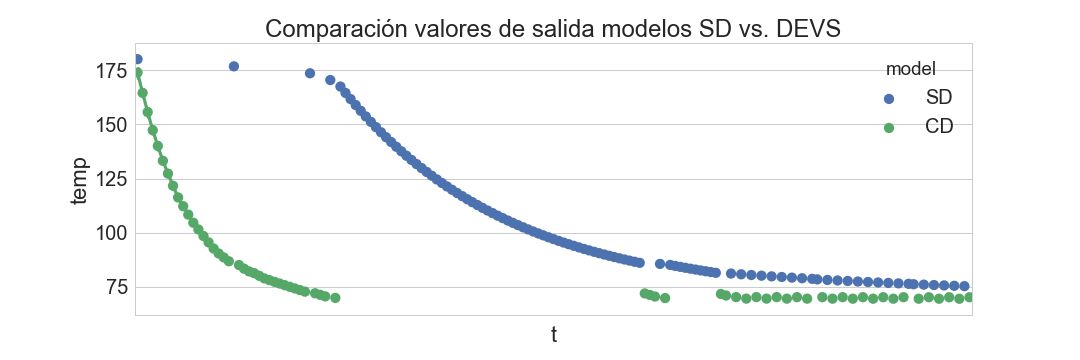
\includegraphics[scale=0.4]{imagenes/tea_comparada_salidas}}
\end{figure}

Si observamos en cambio la salida del modelo \textit{SIR} observamos en las figuras \ref{fig:sir_infect}, \ref{fig:sir_recup} y \ref{fig:sir_sucep} que los valores coinciden en toda la evolución del sistema.

\begin{figure}[H]
    \centering     %%% not \center
    \subfigure[Comparación salida modelo SIR variable: Infectados]{\label{fig:sir_infect}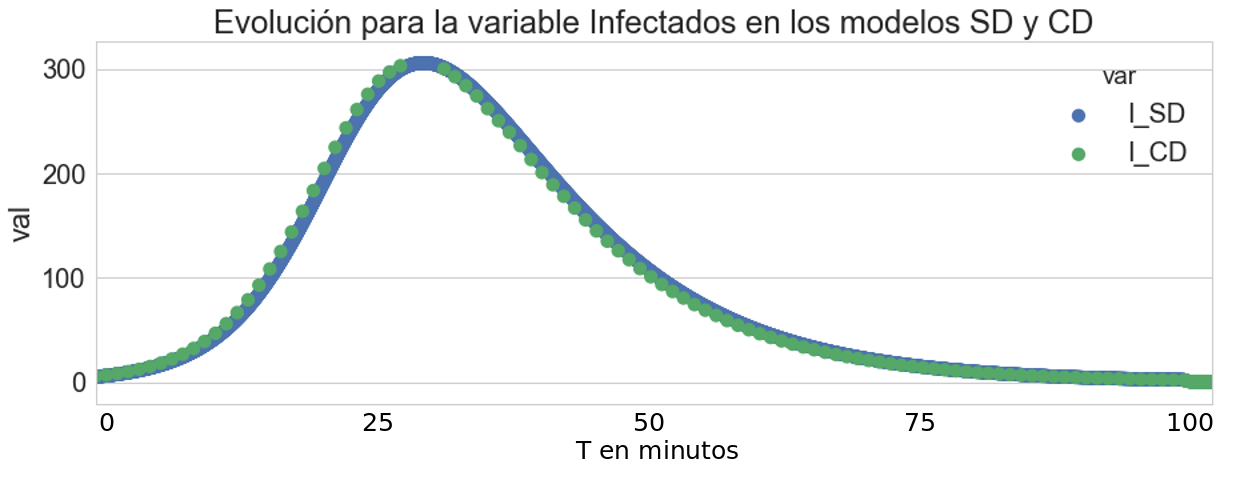
\includegraphics[scale=0.4]{imagenes/sir_comparada_salidas_infectados.png}}
    \subfigure[Comparación salida modelo SIR variable: Recuperandose]{\label{fig:sir_recup}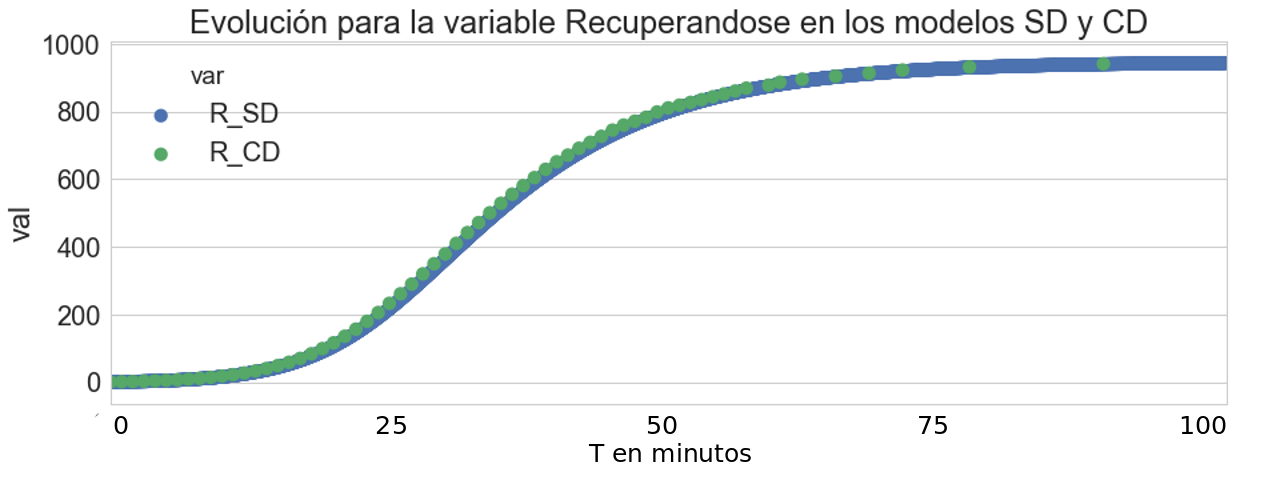
\includegraphics[scale=0.4]{imagenes/sir_comparada_salidas_recuperandose.png}}
    \subfigure[Comparación salida modelo SIR variable: Susceptibles]{\label{fig:sir_sucep}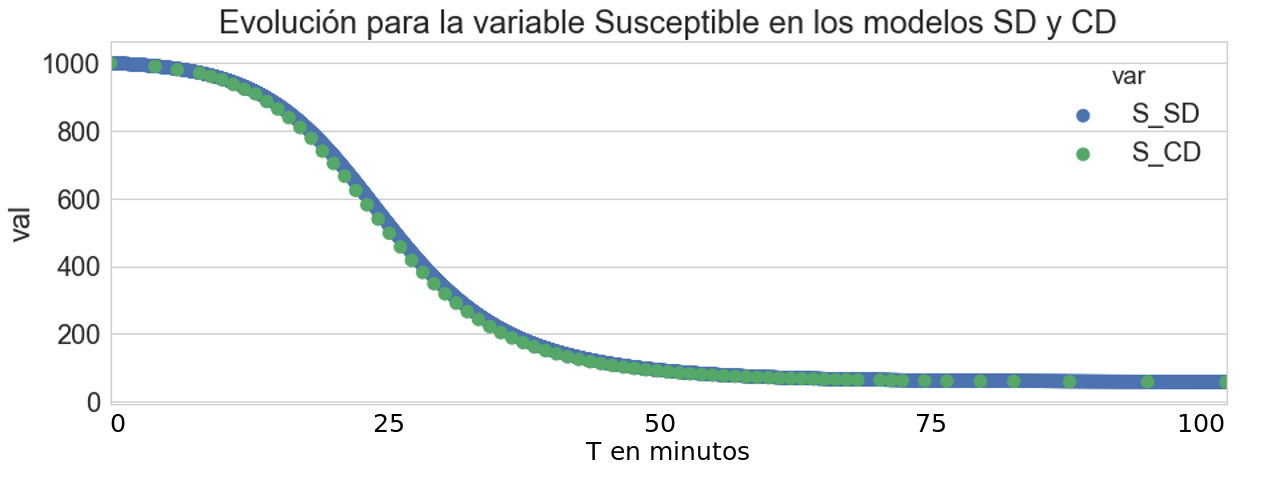
\includegraphics[scale=0.4]{imagenes/sir_comparada_salidas_suseptibles.png}}
        \caption{Modelo SIR - comparación de resultados}
\end{figure}

La granularidad de los dos modelos se explica ya que \textit{CD++} opera de manera discreta mientras que \textit{SD} resuelve el sistema de manera continua.
